\chapter{Introduction}

\par \textbf{Industrial Training} serves as an essential link between academic knowledge and professional work experience. It provides students with the opportunity to apply theoretical concepts learned in the classroom to practical, real-world situations within an organizational setting. This hands-on exposure helps students develop not only technical skills but also important soft skills such as communication, teamwork, and time management, which are vital for success in the professional environment.

\par The primary purpose of industrial training is to prepare students for the workforce by familiarizing them with workplace culture, industry practices, and operational procedures. It enables students to face real challenges, learn problem-solving techniques, and understand the expectations of a professional setting. By engaging in actual projects, interns can bridge the gap between academic theories and industrial applications.

\section{Problem Domain}

\par This industrial training report documents my experiences and learning outcomes during my internship at [Company Name]. During this period, I was involved in [briefly mention area of focus or department, e.g., Software Testing, Marketing, Mechanical Engineering]. As a trainee, I encountered various challenges such as [mention typical issues like unfamiliarity with company tools, adapting to professional workflows, or specific technical difficulties]. Support from supervisors and colleagues helped me overcome these challenges and successfully contribute to assigned tasks.

\section{Motivation of Training}

\par The motivation behind pursuing industrial training includes:

\begin{itemize}
    \item \textbf{Professional Development:} Gaining practical experience and developing relevant skills aligned with the industry.
    \item \textbf{Career Exploration:} Understanding different career paths and industry environments.
    \item \textbf{Application of Knowledge:} Applying academic theories in a practical setting to reinforce learning.
    \item \textbf{Skill Enhancement:} Improving technical, analytical, and interpersonal skills through real work exposure.
    \item \textbf{Adaptability:} Learning to work effectively within a dynamic and evolving workplace.
    \item \textbf{Networking:} Building professional relationships and receiving mentorship.
    \item \textbf{Career Foundation:} Preparing for future employment by gaining hands-on experience and industry insights.
\end{itemize}

\section{Objective of Training}

\par The objectives of this industrial training program are:

\begin{itemize}
    \item To gain practical experience in [mention relevant field, e.g., software quality assurance, marketing strategies].
    \item To develop problem-solving skills through participation in real projects.
    \item To understand and apply industry standards, tools, and best practices.
    \item To improve communication and collaboration skills by working with professionals.
    \item To familiarize myself with current technologies and workflows used in the industry.
    \item To contribute meaningfully to the organization’s goals through assigned tasks.
\end{itemize}

\section{Scope of Training}

\par The scope of this industrial training encompassed activities directly related to [mention specific field or department, e.g., software testing, mechanical design, marketing campaigns]. It included hands-on project work, participation in team meetings, and use of industry-standard tools. Areas outside the core project scope, such as unrelated departments or advanced research work, were not covered. This focus ensured concentrated skill development and meaningful contributions within the assigned domain.


\section{Identifying the Gap Between Academia and Industry}

\par There is often a notable gap between academic learning and industry requirements. Common causes include:

\begin{itemize}
    \item \textbf{Theoretical Knowledge vs Practical Application:} Academic curricula often focus on theory, with limited exposure to practical challenges and real-world constraints.
    \item \textbf{Limited Access to Industry Tools:} Students may not have hands-on experience with current technologies and software widely used in the industry.
    \item \textbf{Work Environment Dynamics:} Academic projects usually lack the collaborative and multidisciplinary teamwork required in professional settings.
    \item \textbf{Standards vs Real-World Constraints:} Industry environments impose deadlines, resource limitations, and changing requirements that are not fully covered in academic programs.
\end{itemize}

\section{Challenges and Areas for Growth}

\subsection{Challenges}
\begin{itemize}
    \item Adapting to a professional work environment and organizational culture.
    \item Balancing project deadlines with thorough task completion.
    \item Overcoming technical challenges related to [mention relevant area].
\end{itemize}

\subsection{Areas for Growth}
\begin{itemize}
    \item Development of practical skills and problem-solving abilities.
    \item Effective time management to meet deadlines.
    \item Exposure to industry-standard tools and technologies.
\end{itemize}


\section{Industrial Training Details Plan}

\par The industrial training was conducted at [Company Name] from [Start Date] to [End Date], focusing on gaining practical experience in [mention field]. During this period, I engaged in various activities aimed at skill enhancement and contributing to organizational objectives.

\subsection{Training Resource Plan}

\begin{enumerate}
    \item \textbf{Human Resources:} Guidance and mentorship from experienced professionals and supervisors provided ongoing support throughout the training.
    \item \textbf{Technical Resources:} Access to relevant tools, software, and hardware necessary for completing assigned tasks effectively.
\end{enumerate}

\subsection{Training Time Management Plan}

\par The training was structured to include orientation, project assignments, evaluations, and feedback sessions spread over the internship period. A timeline similar to Figure \ref{fig:whole_time} was followed to ensure balanced and comprehensive training.

\begin{figure}[H]
    \centering
    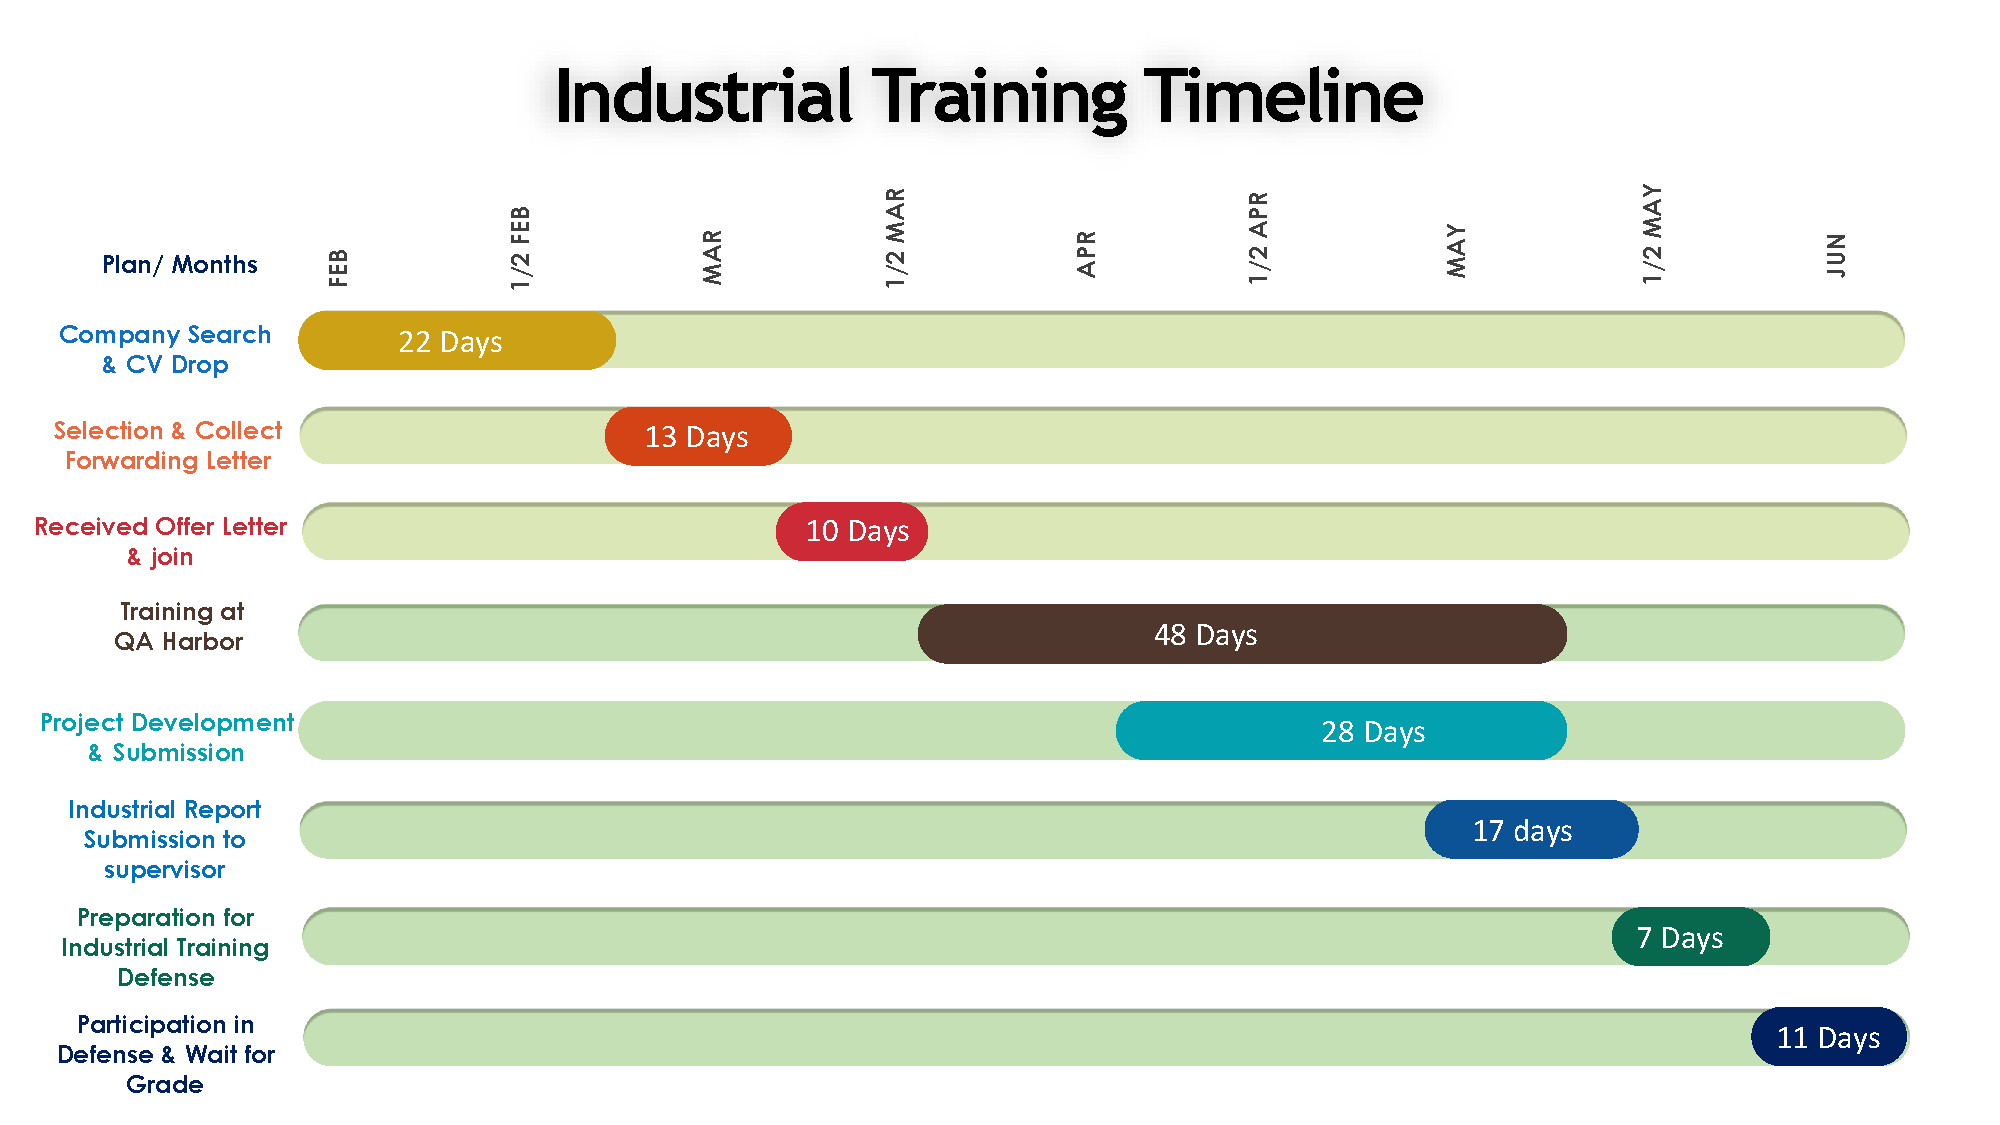
\includegraphics[width=1\linewidth]{figures/Whole Industrial Training Timeline.pdf}
    \caption{Time Management of the Industrial Training Process}
    \label{fig:whole_time}
\end{figure}

\section{Risk Analysis and Resolve Process}

\par During the internship, potential risks such as time constraints, technical difficulties, and communication barriers were identified and managed proactively following a standard risk management process comprising identification, assessment, mitigation, and monitoring (see Figure \ref{fig:risk}).

% 
\textcolor{red}{(You have to refer and describe every Figure you mentioned in your report like above)}

\begin{figure}[H]
    \centering
    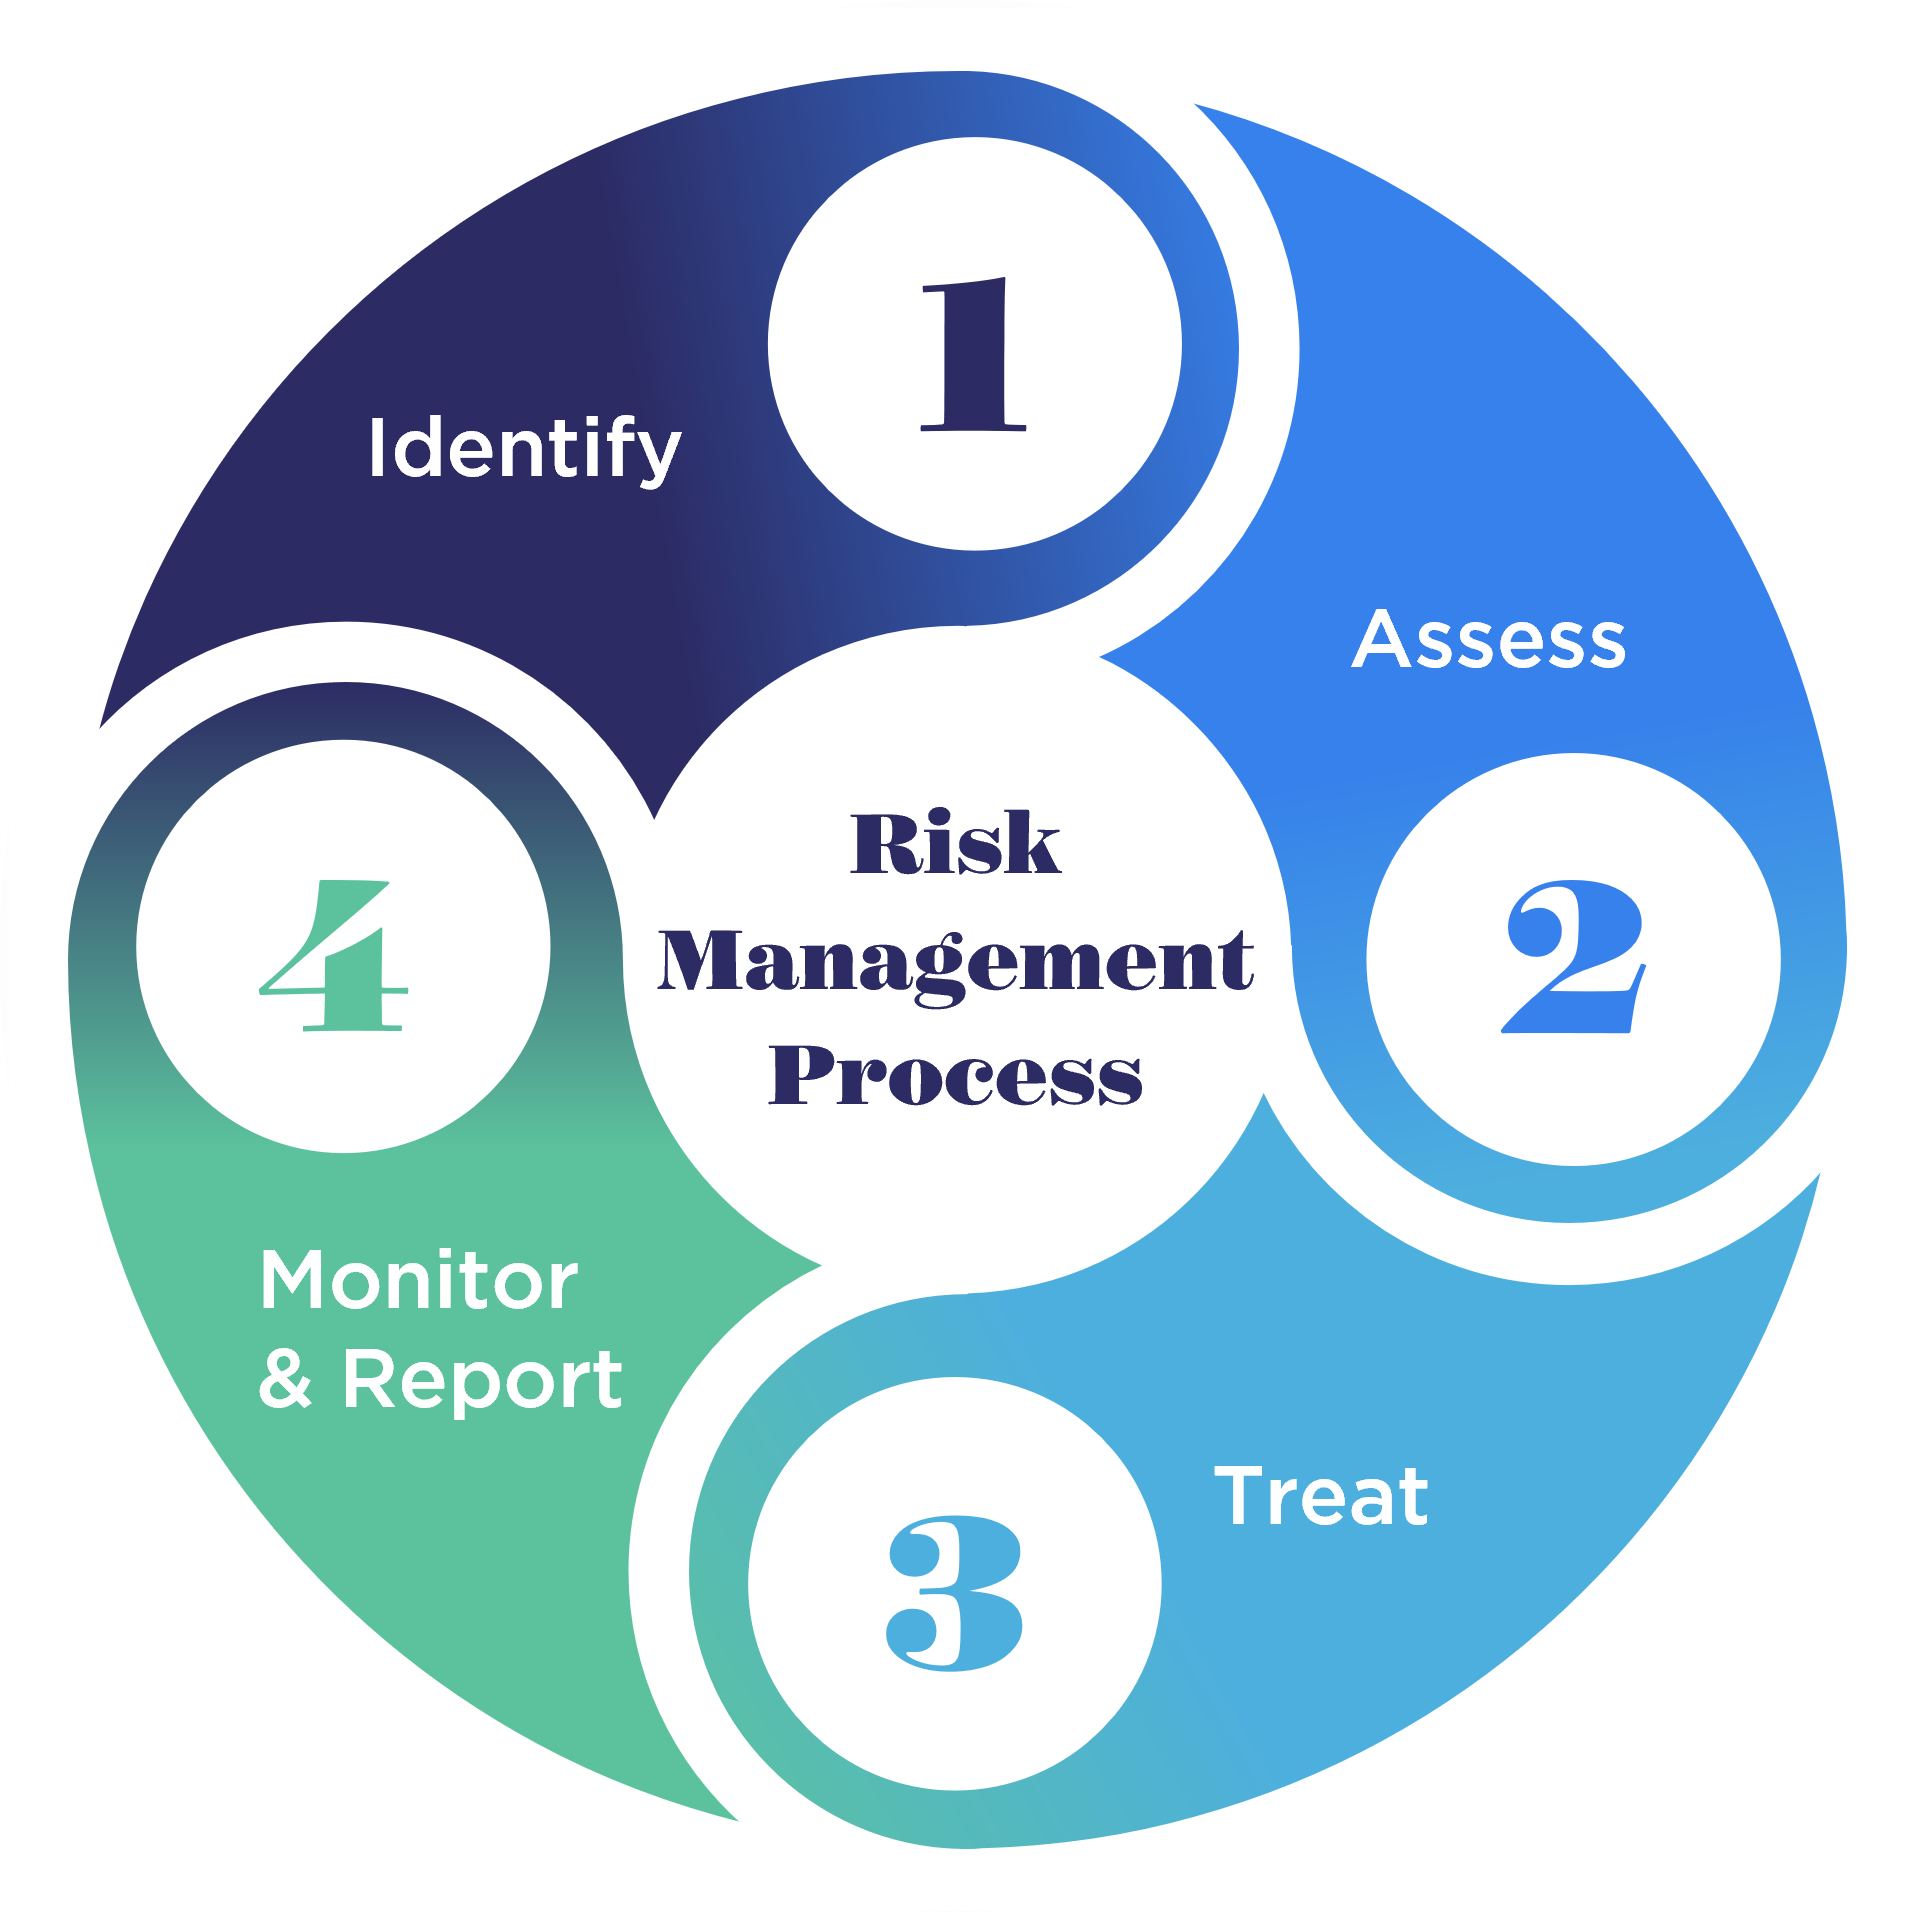
\includegraphics[width=0.3\linewidth]{figures/Four-Steps-of-the-Risk-Management-Process-1 (1).png}
    \caption{Four Steps of the Risk Management Process}
    \label{fig:risk}
\end{figure}

\section{Industrial Training Report Outline}

\begin{itemize}
    \item \textbf{Chapter 2:} Organization Overview – Company structure, services, and mission.
    \item \textbf{Chapter 3:} Training Overview – Key activities, tools, and methodologies applied.
    \item \textbf{Chapter 4:} Skills Acquired – Summary of technical and soft skills developed.
    \item \textbf{Chapter 5:} Conclusion – Reflections, challenges, and recommendations.
\end{itemize}

\section{Conclusion}

\par Industrial training is a vital component in bridging the gap between academic studies and professional work life. It equips students with practical skills, industry exposure, and a better understanding of workplace dynamics. This experience prepares interns for successful careers and enhances their readiness for future challenges in their respective fields.

